\def\duedate{\today}
\def\HWnum{3}
\documentclass[10pt,a4paper]{book}

% custom section formatting
\usepackage{titlesec}
\titleformat{\chapter}[display]
{\normalfont\Large\filcenter\sffamily}
{\titlerule[1pt]%
\vspace{1pt}%
\titlerule
\vspace{1pc}%
\LARGE\MakeUppercase{\chaptertitlename} \thechapter}
{1pc}
{\titlerule
\vspace{1pc}%
\Huge}

% appendix handling
\usepackage[toc,page]{appendix}
    
% encoding for file and font
\usepackage[utf8]{inputenc}
\usepackage[T1]{fontenc}

% math formatting/tools
\usepackage{amsmath}
\usepackage{amssymb}
\usepackage{mathtools}
\usepackage[arrowdel]{physics}

% unit formatting
\usepackage{siunitx}
\AtBeginDocument{\RenewCommandCopy\qty\SI}

% figure formatting/tools
\usepackage{graphicx}
\usepackage{float}
\usepackage{subcaption}
\usepackage{multirow}
\usepackage{import}
\usepackage{pdfpages}
\usepackage{transparent}
\usepackage{currfile}

\NewDocumentCommand\incfig{O{1} m}{
    \def\svgwidth{#1\textwidth}
    \import{./Figures/\currfiledir}{#2.pdf_tex}
}

\newcommand{\bef}{\begin{figure}[h!tb]\centering}
\newcommand{\eef}{\end{figure}}

\newcommand{\bet}{\begin{table}[h!tb]\centering}
\newcommand{\eet}{\end{table}}

% hyperlink references 
\usepackage{hyperref}
\hypersetup{
    colorlinks=true,
    linkcolor=blue,
    filecolor=magenta,
    urlcolor=cyan,
    pdftitle={Physics 1 Notes},
    pdfauthor={Richard Whitehill},
    pdfpagemode=FullScreen
}
\urlstyle{same}

\newcommand{\eref}[1]{Eq.~(\ref{eq:#1})}
\newcommand{\erefs}[2]{Eqs.~(\ref{eq:#1})--(\ref{eq:#2})}

\newcommand{\fref}[1]{Fig.~(\ref{fig:#1})}
\newcommand{\frefs}[2]{Fig.~(\ref{fig:#1})--(\ref{fig:#2})}

\newcommand{\aref}[1]{Appendix~(\ref{app:#1})}
\newcommand{\sref}[1]{Section~(\ref{sec:#1})}
\newcommand{\srefs}[2]{Sections~(\ref{sec:#1})-(\ref{sec:#2})}

\newcommand{\tref}[1]{Table~(\ref{tab:#1})}
\newcommand{\trefs}[2]{Table~(\ref{tab:#1})--(\ref{tab:#2})}

% tcolorbox formatting/definitions
\usepackage[most]{tcolorbox}
\usepackage{xcolor}
\usepackage{xifthen}
\usepackage{parskip}

\definecolor{peach}{rgb}{1.0,0.8,0.64}

\DeclareTColorBox[auto counter, number within=chapter]{defbox}{O{}}{
    enhanced,
    boxrule=0pt,
    frame hidden,
    borderline west={4pt}{0pt}{green!50!black},
    colback=green!5,
    before upper=\textbf{Definition \thetcbcounter \ifthenelse{\isempty{#1}}{}{: #1} \\ },
    sharp corners
}

\newcommand*{\eqbox}{\tcboxmath[
    enhanced,
    colback=black!10!white,
    colframe=black,
    sharp corners,
    size=fbox,
    boxsep=8pt,
    boxrule=1pt
]}

\newtcolorbox[auto counter, number within=chapter]{exbox}{
    parbox=false,
    breakable,
    enhanced,
    sharp corners,
    boxrule=1pt,
    colback=white,
    colframe=black,
    before upper= \textbf{Example \thetcbcounter:}\,,
    before lower= \textbf{Solution:}\,,
    segmentation hidden
}

\newtcolorbox{resbox}{
    enhanced,
    colback=black!10!white,
    colframe=black,
    boxrule=1pt,
    boxsep=0pt,
    top=2pt,
    ams nodisplayskip,
    sharp corners
}


\begin{document}

\prob{1}{

A point charge $q$ is brought to a position a distance $d$ away from an infinite plane conductor held at zero potential.
Using the method of images, find: \\[1pt]

(a) the surface-charge density induced on the plane, and plot it;

(b) the force between the plane and the charge by using Coulomb's law for the force between the charge and its image;

(c) the total force acting on the plane by integrating $\sigma^2 / 2 \epsilon_0$ over the whole plane;

(d) the work necessary to remove the charge $q$ from its position to infinity;

(e) the potential energy between the charge $q$ and its image [compare the answer to part(d) and discuss];

(f) Find the answer to part (d) in electron volts for an electron originally one angstrom from the surface.

}

\begin{figure}[h!]
   \centering
   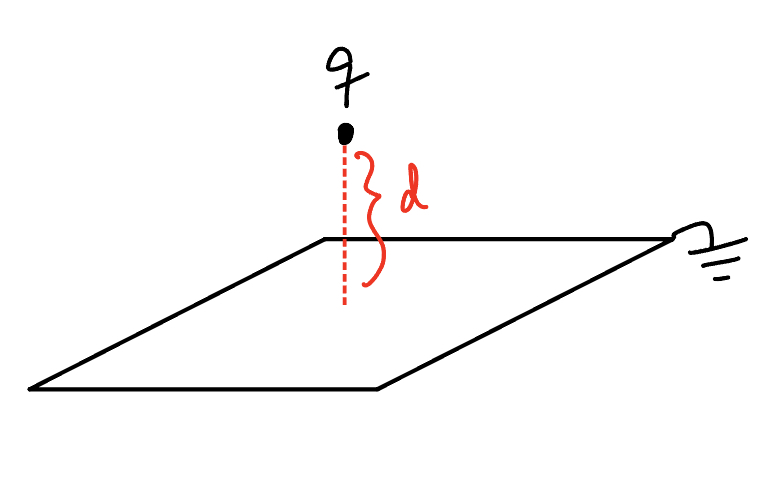
\includegraphics[width=0.4\textwidth]{prob1.jpeg}
   \caption{Sketch of setup with charge $q$ brought to a distance $d$ from an infinite grounded, conducting plane.}
   \label{fig:prob1}
\end{figure}

\sol{

(a) Solving this problem using the method of images, we place an image charge $-q$ on the other side of the plane a distance $d$ away.
The potential of this setup is
\begin{eqnarray}
    \Phi(\va*{r}) = \frac{q}{4 \pi \epsilon_0} \Bigg( \frac{1}{|\va*{r} - d \vu*{e}_{z}|} - \frac{1}{|\va*{r} + d \vu*{e}_{z}|} \Bigg)
.\end{eqnarray}
We know that this is the correct potential since it satisfies Laplace's equation for $z > 0$ (defining the $z$-axis perpendicular to the plane and the $+$ direction pointing from the plane to the charge $q$) and the boundary conditions $\Phi(x,y,0) = 0$.

The relation between the potential and surface charge density is
\begin{eqnarray}
    \eqbox{
    \begin{aligned}
        \sigma &= -\epsilon_0 \pdv{\Phi}{z} = \frac{q}{4 \pi} \pdv{z} \Bigg( \frac{1}{\sqrt{x^2 + y^2 + (z - d)^2}} - \frac{1}{\sqrt{x^2 + y^2 + (z + d)^2}} \Bigg)_{z = 0} \\
               &= -\frac{q}{4 \pi} \Bigg( \frac{-(z - d)}{[ x^2 + y^2 + (z - d)^2 ]^{3/2}} - \frac{- (z + d)}{[ x^2 + y^2 + (z + d)^2 ]^{3/2}} \Bigg)_{z = 0} \\
               &= - \frac{qd}{2 \pi (\rho^2 + d^2)^{3/2}}
    ,\end{aligned}
}
\end{eqnarray}
where we have defined $\rho^2 = x^2 + y^2$.
Notice that the induced charge has an overall charge with sign opposite that of $q$.

\begin{figure}[h!]
   \centering
   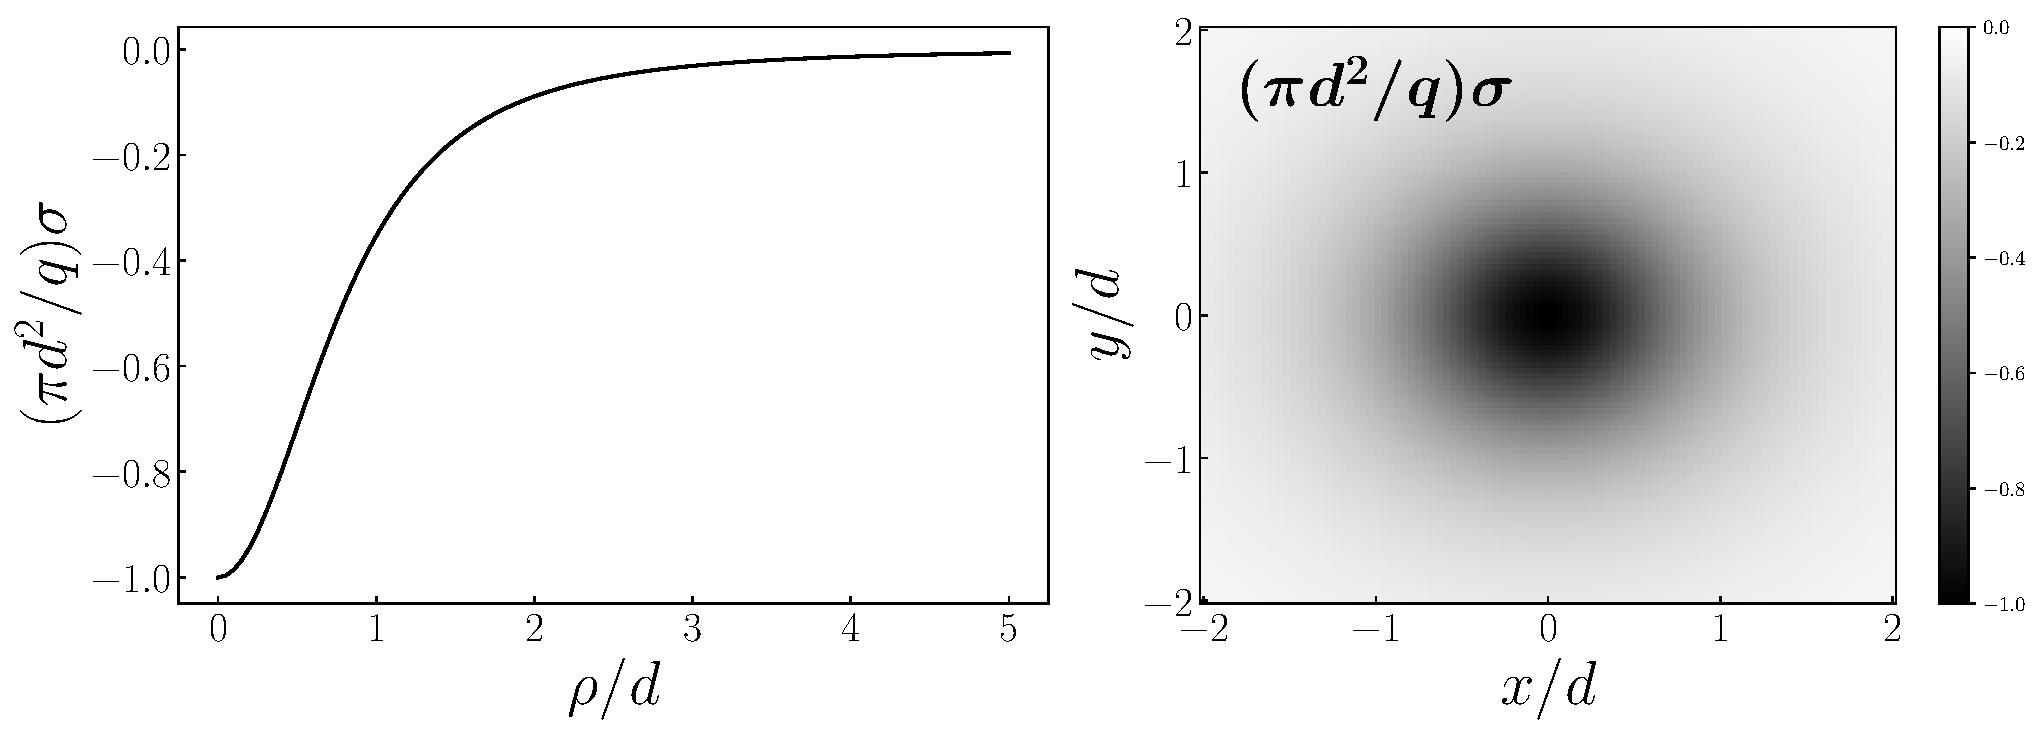
\includegraphics[width=\textwidth]{prob1a.pdf}
   \caption{\textbf{Left} -- Plot of surface charge density with respect to spatial variable $\rho = \sqrt{x^2 + y^2}$ and \textbf{Right} -- Plot of surface charge density with respect to $(x,y)$ coordinates. Note that the spatial variables are in units of $d$, and furthermore, in the colormap plot on the right, one can intuitively read this to say that more charge aggregates directly below the charge $q$ and the distribution falls off radially from this center.}
   \label{fig:prob1a}
\end{figure}

(b) The force between the plane and point charge $q$ can be calcualted using Coulomb's law between $q$ and $-q$
\begin{eqnarray}
    \eqbox{ \va*{F} = - \frac{q^2}{4 \pi \epsilon_0} \frac{1}{(2d)^2} }
.\end{eqnarray}

(c) We can also calculate the total force acting on the plane as follows:
\begin{eqnarray}
    \eqbox{
   \begin{aligned}
       F &= \int \frac{\sigma^2(x,y)}{2 \epsilon_0} \dd{x} \dd{y} = \frac{q^2 d^2}{8 \pi^2 \epsilon_0} \int_{0}^{2 \pi} \int_{0}^{\infty} \frac{1}{(\rho^2 + d^2)^3} \rho \dd{\rho} \dd{\phi} \\
         &= \frac{q^2 d^2}{4 \pi \epsilon_0} \int_{0}^{\infty} \frac{\rho}{(\rho^2 + d^2)^3} \dd{\rho} = -\frac{q^2 d^2}{4 \pi \epsilon_0} \frac{1}{4 d^{4}} = -\frac{q^2}{4 \pi \epsilon_0} \frac{1}{(2d)^2}
   .\end{aligned} 
}
\end{eqnarray}
Also, it should be clear that the force is attractive.

(d) From part (b), we can calculate the work needed to move the charge $q$ infinitely far from the plane as follows
\begin{eqnarray}
    \eqbox{ W = \int_{d}^{\infty} \frac{q^2}{4 \pi \epsilon_0} \frac{1}{(2 z)^2} \dd{z} = \frac{q^2}{4 \pi \epsilon_0} \frac{1}{4 d} }
.\end{eqnarray}
Note that the sign is correct since we have to apply a force opposing the attractive force between the plane and charge.

(e) The potential energy between the charge $q$ and its image charge $-q$ is 
\begin{eqnarray}
    U = q \Phi_{-}(d \vu*{e}_{z}) = - \frac{q^2}{4 \pi \epsilon_0} \frac{1}{2 d} = -2 W
,\end{eqnarray}
where $\Phi_{-}$ is the potential due to the image charge $-q$.
Note that this result is twice the work it takes to construct this system.
One can imagine setting up the image charge distribution by moving both charges in from infinity symmetrically, but since the image charge is virtual, it does not contribute anything to the work done.
Hence, the actual work done to place the charge $q$ at distance $d$ from the plane is only half that to set up the dipole image distribution.
Alternatively, one can see that there is not work done on the plane when the charge $q$ is brought in since it is held at $\Phi \equiv 0$, and the image charge assumes the role of the plane in the image.

(f) For an electron ($q \approx 1.602 \times 10^{-19}~{\rm C}$) a distance $d = 1~{\textrm{\r{A}}}$ away from the plane initially, the work done to move it to $\infty$ is
\begin{eqnarray}
    \eqbox{ W \approx 3.6~{\rm eV} }
.\end{eqnarray}


}


\prob{2}{

Using the method of images, discuss the problem of a point charge $q$ inside a hollow, grounded, conducting sphere of inner radius $a$.
Find \\[1pt]

(a) the potential inside the sphere;

(b) the induced surface-charge density;

(c) the magnitude and direction of the force acting on $q$.

(d) Is there any change in the solution if the sphere is kept at a fixed potential $V$?
If the sphere has a total charge $Q$ on its inner and outer surfaces?

}

\begin{figure}[h!]
   \centering
   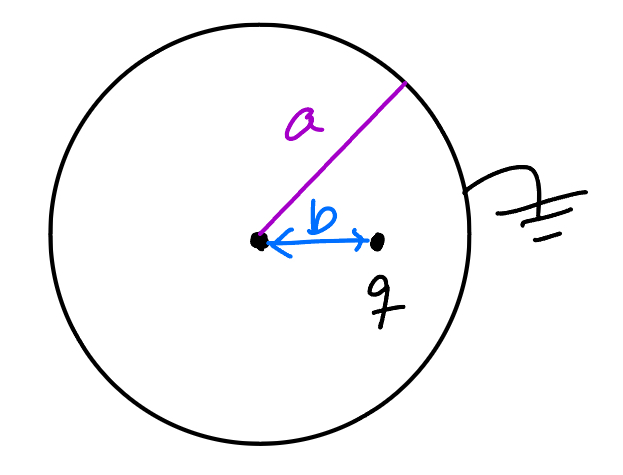
\includegraphics[width=0.3\textwidth]{prob2.jpeg}
   \caption{Sketch of problem setup with charge $q$ at the center of a hollow, conducting, grounded sphere of radius $a$.}
   \label{fig:prob2}
\end{figure}

\sol{

(a) We have addressed the problem of a charge outside the sphere and solved by placing an image charge inside the sphere.
In this case, we just reverse the role of the charge and image charges.
The potential inside the sphere is therefore
\begin{eqnarray}
    \eqbox{ \Phi(\va*{r}) = \frac{1}{4 \pi \epsilon_0} \Bigg[ \frac{q}{|\va*{r} - \va*{b}|} + \frac{q'}{|\va*{r} - \va*{b}'|} \Bigg] }
,\end{eqnarray}
where $q' = -(a/b) q$ and $\va*{b}' = (a/b)^2 \va*{b}$.

(b) We can find the induced surface-charge density from the electric field at the surface of the sphere, which is 
\begin{eqnarray}
    \begin{aligned}
        \va*{E} &= \frac{q}{4 \pi \epsilon_0} \Bigg[ \frac{a \vu*{e}_{r} - \va*{b}}{| a \vu*{e}_{r} - \va*{b} |^3} - \frac{a}{b} \frac{a \vu*{e}_{r} - \va*{b}'}{| a \vu*{e}_{r} - \va*{b}' |^3} \Bigg] = \frac{q}{4 \pi \epsilon_0} \Bigg[ \frac{a \vu*{e}_{r} - \va*{b}}{|a \vu*{e}_{r} - b \vu*{e}_{x}|^3} - \frac{a}{b} \frac{a \vu*{e}_{r} - (a/b)^2 \va*{b}}{|a \vu*{e}_{r} - (a^2/b) \vu*{e}_{x}|^3} \Bigg] \\
                &= \frac{q}{4 \pi \epsilon_0} \Bigg[ \frac{a \vu*{e}_{r} - \va*{b}}{b^3|(a/b)\vu*{e}_{r} - \vu*{e}_{x}|^3} - \frac{a}{b} \frac{a \vu*{e}_{r} - (a/b)^2 \va*{b}}{a^3|\vu*{e}_{r} - (a/b) \vu*{e}_{x}|^3} \Bigg] \\
                &= \frac{q}{4 \pi \epsilon_0 b^2} \frac{1}{[1 + (a/b)^2 - 2(a/b)\cos{\theta}]^{3/2}} \Bigg[ \Big( \frac{a}{b} \vu*{e}_{r} - \vu*{e}_{x} \Big) - \frac{1}{b} \Big( \frac{b^2}{a} \vu*{e}_{r} - \vu*{e}_{x} \Big) \Bigg] \\
                &= \frac{q}{4 \pi \epsilon_0 b^2} \Big( \frac{a}{b} \Big) \frac{1 - (b/a)^2}{[1 + (a/b)^2 - 2(a/b) \cos{\theta}]^{3/2}} \vu*{e}_{r} \\
                &= - \frac{q}{4 \pi \epsilon_0 a^2} \Big( \frac{a}{b} \Big) \frac{1 - (a/b)^2}{[1 + (a/b)^2 - 2(a/b)\cos{\theta}]^{3/2}} \vu*{e}_{r}
    .\end{aligned}
\end{eqnarray}
The surface charge density is then given as
\begin{eqnarray}
    \eqbox{ \sigma = \epsilon_0 \va*{E} \cdot (- \vu*{e}_{r}) = \frac{q}{4 \pi \epsilon_0 a^2} \Big( \frac{a}{b} \Big) \frac{1 - (a/b)^2}{[1 + (a/b)^2 - 2(a/b) \cos{\theta}]^{3/2}} }
.\end{eqnarray}

(c) The magnitude of the force on $q$ is just
\begin{eqnarray}
    \eqbox{ F = \frac{|q q'|}{4 \pi \epsilon_0 (b' - b)^2} = \frac{q^2}{4 \pi \epsilon_0 b^2} \Big( \frac{a}{b} \Big) [1 - (a/b)^2]^{-2} = \frac{q^2}{4 \pi \epsilon_0 a^2} \Big( \frac{a}{b} \Big)^3 [1 - (a/b)^2]^{-2} }
\end{eqnarray}
and points away from the center of the sphere (i.e. toward the surface of the sphere in the $\vu*{e}_{x}$ direction).

(d) If we hold the sphere at potential $V$, this is equivalent to shifting our ground to infinity such that our potential is changed by $V(a/r)$ outside the sphere.
That is, holding the sphere to potential $V$ is equivalent to placing charge $4 \pi \epsilon_0 (a V)$ on the sphere.
Hence, the potential inside the sphere is shifted by $V$, but the induced surface charge density is left unchanged as is the force on $q$ since the electric field from this surface charge is zero inside the sphere.

Placing total charge $Q$ on the inner and outer surfaces of the sphere does not change the results in a significant way by the same reasoning as in the previous paragraph.

}


\prob{3}{

    A point charge is placed a distance $d > R$ from the center of an equally charged, isolated, conducting sphere of radius $R$. \\[1pt]

(a) Inside of what distance from the surface of the sphere is the point charge attracted rather than repelled by the charged sphere?

(b) What is the limiting value of the force of atrraction when the point charge is located a distance $a = d - R$ from the surface of the sphere, if $a \ll R$?

(c) What are the results for parts (a) and (b) if the charge on the sphere is twice (half) as large as the point charge, but still the same sign?

}

\begin{figure}[h!]
   \centering
   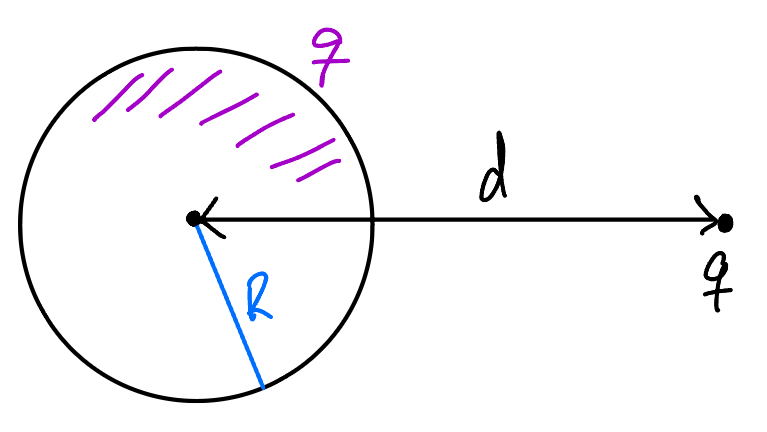
\includegraphics[width=0.3\textwidth]{prob3.jpeg}
   \caption{Sketch of problem setup with charge $q$ a distance $d$ from the center of a sphere of radius $R$ with surface charge $q$.}
   \label{fig:prob3}
\end{figure}

\sol{

(a) We can solve this problem by placing image charges $q'$ a distance $x$ from the center of the sphere and a charge $\hat{q}$ at the center of the sphere, where $q' + \hat{q} = q$, where $q$ is the total charge placed on the sphere.
The potential outside the sphere (i.e. $r > R$) for this setup is
\begin{eqnarray}
    \Phi(\va*{r}) = \frac{1}{4 \pi \epsilon_0} \Bigg[ \frac{q}{|\va*{r} - \va*{d}|} + \frac{q'}{|\va*{r} - \va*{x}|} + \frac{\hat{q}}{r} \Bigg]
.\end{eqnarray}
Note that $q' = -(R/d) q$ and $x = R^2/d$.
This implies that the force on the charge $q$ is
\begin{eqnarray}
    \begin{aligned}
        F &= \frac{q}{4 \pi \epsilon_0} \Big[ \frac{q'}{(d - x)^2} + \frac{zq - q'}{d^2} \Big] = \frac{q^2}{4 \pi \epsilon_0} \Bigg[ -\frac{R}{d} \frac{1}{(d - R^2/d)^2} + \frac{1 + R/d}{d^2} \Bigg] \\
          &= \frac{q^2}{4 \pi \epsilon_0 d^2} \Bigg[ -\frac{R}{d} \frac{1}{(1 - (R/d)^2 )^2} + 1 + \frac{R}{d} \Bigg] = \frac{q^2}{4 \pi \epsilon_0 d^2} \Bigg[ \frac{R}{d} \Bigg( 1 - \frac{1}{(1 - (R/d)^2)^2} \Bigg) + 1 \Bigg] \\
          &= \frac{q^2}{4 \pi \epsilon_0 d^2} \Bigg[ 1 - \frac{R^3(2 d^2 - R^2)}{d(d^2 - R^2)^2} \Bigg]
    \end{aligned}
\end{eqnarray}
directed along the line from the center of the sphere to the charge $q$.
Thus,
\begin{eqnarray}
    \label{eq:F-neg-cond}
    F < 0 \Rightarrow \frac{R^3(2 d^2 - R^2)}{d(d^2 - R^2)^2} > 1 
.\end{eqnarray}
To solve this, let us first change to the dimensionless variable $x = d/R$.
\eref{F-neg-cond} then reads
\begin{eqnarray}
    \label{eq:F-neg-cond-x}
    \frac{2x^2 - 1}{x(x^2 - 1)^2} > 1
.\end{eqnarray}
Next, we will write $a = d - R = (x - 1) R$ and define $\xi = x - 1$ such that \eref{F-neg-cond} reads
\begin{eqnarray}
    \frac{2 \xi^2 + 4 \xi + 1}{\xi^{5} + 5\xi^{4} + 8\xi^3 + 4 \xi^2} > 1 
\end{eqnarray}
in terms of $\xi$.

Observe that this gives $P_{5}(\xi) > 0$, where $P_{5}$ is a $5^{\rm th}$ order polynomial.
Since this does not simplify any further analytically (at least in a way that is obvious in its current form), we will solve the problem numerically\footnote{As a practical note, we will solve \eref{F-neg-cond-x} first and subtract one from the result since this is more compact.}.
Here, we are concerned with $z = 1$, which gives $\eqbox{ \xi = d/R - 1 \lesssim 0.618 }$.

(b) We want the limiting behavior of the force on the point charge when $a \ll R$.
In other words, we will exand $F$ in powers of $\xi = a/R$ and keep only the leading non-vanishing term:
\begin{eqnarray}
    \eqbox{ F \approx \frac{q^2}{4 \pi \epsilon_0 R^2} \Bigg[ 1 - \frac{1}{4 \xi^2} \Bigg] \approx -\frac{q^2}{16 \pi \epsilon_0 R^2} \frac{R^2}{a^2} = -\frac{q^2}{16 \pi \epsilon_0 a^2} = -\frac{q^2}{4 \pi \epsilon_0 (2 a)^2} }
.\end{eqnarray}

(c) If the charge on the sphere is $Q$, then the force on the charge is given as
\begin{eqnarray}
    F = \frac{q^2}{4 \pi \epsilon_0} \Bigg[ (Q/q) - \frac{R^3(2 d^2 - R^2)}{d(d^2 - R^2)^2} \Bigg]
.\end{eqnarray}
Thus, the condition for the turning point between the charge $q$ feeling an attractive and repulsive force is modified to
\begin{eqnarray}
    \frac{R^3(2 d^2 - R^2)}{d(d^2 - R^2)^2} > Q/q
,\end{eqnarray}
and therefore
\begin{eqnarray}
    \eqbox{
    \xi \approx \begin{cases}
        0.428 & {\rm if}~Q/q = 2 \\
        0.882 & {\rm if}~Q/q = 1/2
    .\end{cases}
}
\end{eqnarray}

Notice, however, that the force on $q$ very near the surface of the sphere is left unchanged.
The first term is constant in $a/R$ while the second is of order $(R/a)^2$, so the second term dominates in this region independent of the value of $Q/q$.
Intuitively, this can be rationalized as follows: the force on $q$ near the surface of the sphere is identical to that of the situation where $q$ is a distance $a$ from an infinite, grounded plane.
That is, there is a significant induced charge on the plane near $q$ when $a \ll R$, which dominates over any other contributions to the force on $q$ overall.

}


\prob{4}{

(a) Show that the work done to remove the charge $q$ from a distance $r > a$ to infinity against the force, Eq. (2.6) in \textit{Jackson} textbook, of a grounded conducting sphere is 
\begin{eqnarray}
   W = \frac{q^2 a}{8 \pi \epsilon_0  (r^2 - a^2)} 
.\end{eqnarray}
Relate this result to the electrostatic potential, Eq. (2.3) in \textit{Jackson} textbook, and the energy discussion of Section 6.3 in Lecture 4.

(b) Repeat the calculation of the work done to remove the charge $q$ against the force, Eq. (2.9) in \textit{Jackson} textbook (see also Section 9.3.3 of Lecture 6), of an isolated charged conducting sphere.
Show that the work done is
\begin{eqnarray}
    W = \frac{1}{4 \pi \epsilon_0} \Big[ \frac{q^2 a}{2 (r^2 - a^2)} - \frac{q^2 a}{2 r^2} - \frac{q Q}{r} \Big]
.\end{eqnarray}
Relate the work to the electrostatic potential, Eq. (2.8) in \textit{Jackson} textbook (see also Section 9.3.2 of Lecture 6), and the energy discussion of Section 6.3 in Lecture 4.

}

\sol{

(a) The work needed to move a charge $q$ from $r > a$ to infinity in the presence of a grounded conducting sphere is
\begin{eqnarray}
    \eqbox{
    \begin{aligned}
        W &= \int_{r}^{\infty} \frac{1}{4 \pi \epsilon_0} \frac{q^2}{a^2} \Big( \frac{a}{x} \Big)^3 \Big( 1 - \frac{a^2}{x^2} \Big)^{-2} \dd{x} = \frac{q^2 a}{4 \pi \epsilon_0} \int_{r}^{\infty} \frac{x}{(x^2 - a^2)^2} \dd{x} \\
        &= \frac{q^2 a}{4 \pi \epsilon_0} \Big( \frac{1}{2} \Big) \int_{r^2 - a^2}^{\infty} \frac{\dd{u}}{u} = \frac{q^2 a}{8 \pi \epsilon_0 (r^2 - a^2)}
    \end{aligned} 
    }
.\end{eqnarray}
Observe that the work $W = -q \Phi'(\va*{r})/2 \sqrt{r^2 - a^2}$, which is similar to the result of problem 1 by the same rational (i.e. only work is being done on $q$ to assemble the configuration).

(b) The work needed to move a charge $q$ from $r > a$ to infinity in the presence of an isolated, conducting sphere with charge $Q$ on it is given by the following
\begin{eqnarray}
    \begin{aligned}
        W &= -\frac{q}{4 \pi \epsilon_0} \int_{r}^{\infty} \Bigg[ \frac{Q}{x^2} - \frac{q a^3 (2 x^2 - a^2)}{x^3 (x^2 - a^2)^2} \Bigg] \dd{x} \\
        &= -\frac{q Q}{4 \pi \epsilon_0 r} + \frac{q^2}{4 \pi \epsilon_0 a} \int_{r/a}^{\infty} \frac{2y^2 - 1}{y^3(y^2 - 1)^2} \dd{y}
    \end{aligned}
,\end{eqnarray}
where in the second integration we have substituted $x = ay$.
Note that we can substitute $u = x^2$ such that 
\begin{eqnarray}
    I = \int_{r/a}^{\infty} \frac{2x^2 - 1}{x^3(x^2 - 1)^2} \dd{x} = \frac{1}{2} \int_{(r/a)^2}^{\infty} \frac{2u - 1}{u^2(u-1)^2} \dd{u}
.\end{eqnarray}
Next, we can substitute $v = u(u-1) = u^2 - u$ such that 
\begin{eqnarray}
    \label{eq:label}
    I = \frac{1}{2} \int_{(r/a)^2((r/a)^2 - 1)}^{\infty} \frac{\dd{v}}{v^2} = \frac{1}{2(r/a)^2[(r/a)^2 - 1]} = -\frac{a^2}{2r^2} + \frac{a^2}{2(r^2 - a^2)}
,\end{eqnarray}
where for the last inequality we have used partial fraction expansion to rewrite the result.
Putting this back
\begin{eqnarray}
    \eqbox{ W = \frac{1}{4 \pi \epsilon_0} \Big[ \frac{q^2 a}{2(r^2 - a^2)} - \frac{q^2 a}{2 r^2} - \frac{qQ}{r} \Big] }
.\end{eqnarray}

This scenario is similarly analyzed as in the previous case.
The first term is exactly that found in part (a), and the third term is the potential energy between charge $Q$ and $q$.
However, the second term comes from the potential of the induced charge density on the sphere and the charge $q$, which is precisely half the energy of the configuration between $q$ and $q'$ if $q'$ were a real charge.

}



\end{document}
